\begin{frame}[standout]

    Bases de données orientées graphe

\end{frame}

\begin{frame}{Caractéristiques des bases de données graphe}

    \begin{definitionbox}
        Dans une base de données graphe, les données sont organisées en \textbf{nœuds}, \textbf{liens} et \textbf{propriétés} qui permettent de modéliser des relations complexes et dynamiques entre les entités. Les \textbf{nœuds} représentent les entités, les \textbf{liens} représentent les relations entre ces nœuds, et les \textbf{propriétés} fournissent des informations supplémentaires sur les nœuds et les liens.
    \end{definitionbox}

    \begin{noteblock}
        \begin{itemize}
            \item Représentation des relations complexes entre les données.
            \item Optimisé pour les requêtes de lecture et les opérations relationnelles.
        \end{itemize}
        % $\Longrightarrow$ Idéal pour des applications nécessitant des relations complexes et dynamiques entre les données.
        $\hookrightarrow$ Idéal pour des applications nécessitant des relations complexes et dynamiques entre les données.
    \end{noteblock}
\end{frame}

\begin{frame}{Bases de données graphe}
    \begin{figure}[htb]
        \centering
        \begin{tikzpicture}
            \node[minimum width=3cm, minimum height=2cm] at (0, 0) {\includesvg[height=1cm]{img/db/neo4j.svg}};
            \node[minimum width=3cm, minimum height=2cm] at (4, 0) {\includesvg[height=0.8cm]{img/db/arangodb.svg}};
            \node[minimum width=3cm, minimum height=2cm] at (0, -3) {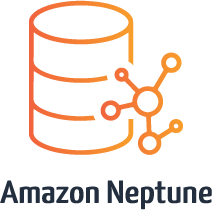
\includegraphics[height=1.3cm]{img/db/aws-neptune.png}};
            \node[minimum width=3cm, minimum height=2cm] at (4, -3) {\includesvg[height=1.3cm]{img/db/orientdb.svg}};
        \end{tikzpicture}
    \end{figure}
\end{frame}

\begin{frame}{Comment fonctionnent les bases de données graphe ?}

    \begin{figure}
        \centering
        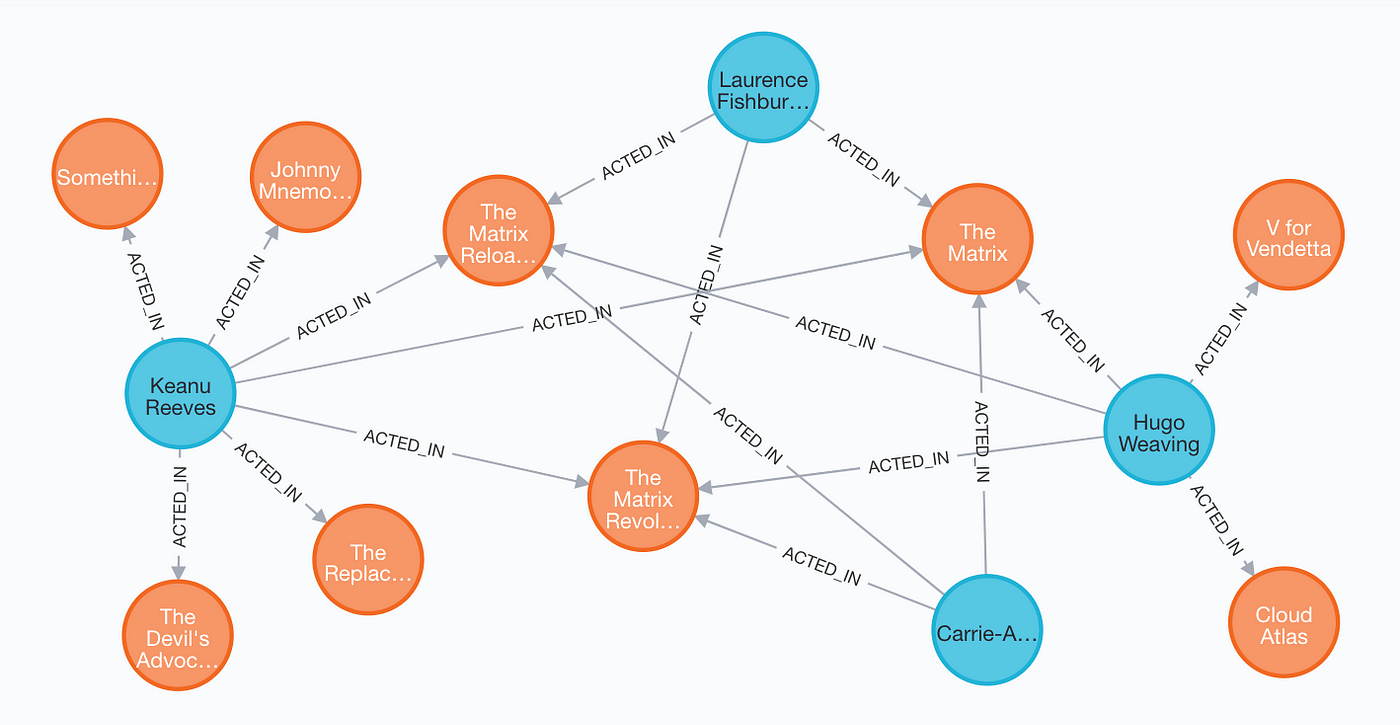
\includegraphics[width=0.8\textwidth]{img/neo4j-graph.png}
    \end{figure}

\end{frame}

\begin{frame}{Cas d'usages des bases de données graphe}

    \begin{itemize}
        \item \textbf{Réseaux sociaux}\\
        $\hookrightarrow$ Modélisation des relations entre utilisateurs, amis, groupes, et interactions pour des recommandations et des analyses sociales.
        \vspace{0.3cm}

        \item \textbf{Détection de fraude}\\
        $\hookrightarrow$ Analyse des connexions entre transactions et entités pour identifier des schémas de fraude ou des comportements suspects.
        \vspace{0.3cm}

        \item \textbf{Systèmes de recommandation}\\
        $\hookrightarrow$ Analyse des préférences des utilisateurs et des relations entre produits pour fournir des recommandations personnalisées.
        \vspace{0.3cm}

        \item \textbf{Gestion des réseaux de télécommunications}\\
        $\hookrightarrow$ Modélisation des réseaux de télécommunications et des relations entre équipements pour optimiser les performances et la maintenance.
    \end{itemize}
\end{frame}

\begin{frame}{Avantages et inconvénients des bases de données graphe}
    \vfill
    \prosbox{
        \textbf{Avantages}
        \begin{itemize}
            \item Excellente performance pour les requêtes impliquant des relations complexes.
            \item Flexibilité pour modéliser des structures de données dynamiques.
        \end{itemize}
    }
    \vfill
    \pause
    \consbox{
        \textbf{Inconvénients}
        \begin{itemize}
            \item Moins efficace pour les opérations non liées aux relations.
            \item Complexité accrue pour les utilisateurs non familiers avec la modélisation en graphe.
        \end{itemize}
    }
    \vfill
\end{frame}


\begin{frame}{Focus sur Neo4j}

\end{frame}

\begin{frame}{Étude de cas}

    LinkedIn et Neo4j (recommandations de connexions).

    Problématique.
    Solution NoSQL choisie.
    Architecture mise en place.
    Résultats (performances, coûts).

\end{frame}
